\documentclass[a4paper,11pt]{article}

\usepackage[margin=2.5cm]{geometry}
\usepackage{amsmath}
\usepackage{tikz}
\usepackage{graphicx}
\usepackage{xcolor}
\usepackage[hidelinks]{hyperref}
\usepackage[backend=biber,style=numeric,sorting=none]{biblatex}
\usetikzlibrary{positioning, arrows.meta}

\addbibresource{references.bib}

\begin{document}

% =====================================================================
% Cover page
% =====================================================================
\begin{titlepage}
    \centering
    \vspace*{2cm}

    {\Large RWTH Aachen University \par}
    {\large Process and Data Science (PADS) \par}

    \vfill

    {\Huge\bfseries State Based Process Monitoring \\[0.3cm] in Traditional Event Logs \\[0.3cm] for Concept Drift Detection \par}

    \vspace{1cm}
    {\Large Bachelor's Thesis \par}

    \vfill

    \begin{tabular}{rl}
        \textbf{Author:}            & Bora Deren \\[0.4em]
        \textbf{Supervisor:}        & Alessandro Berti \\[0.4em]
        \textbf{First examiner:}    & Prof.\ Dr.\ Wil van der Aalst \\
    \end{tabular}

    \vfill

    {\large \today \par}
\end{titlepage}

\tableofcontents
\newpage

% =====================================================================
\section{Introduction}
Placeholder.

% =====================================================================
\section{Related Work}
Placeholder.

% =====================================================================
\section{Background}
Placeholder.

% =====================================================================
\section{State Types}

This thesis defines three complementary state types for traditional event logs,
inspired by~\cite{berti2025ocel}.

\subsection{Intra-case State}
Placeholder.

\subsection{Resource State}
Placeholder.

\subsection{Inter-case State}
Placeholder.

% =====================================================================
\section{Approach}

\subsection{Feature Extraction}
Placeholder.

\subsection{Dimensionality Reduction}
Placeholder.

\subsection{State Discovery}
Placeholder.

\subsection{Drift Detection}
Placeholder.

\subsection{Pipelines}

\begin{figure}[ht]
\centering
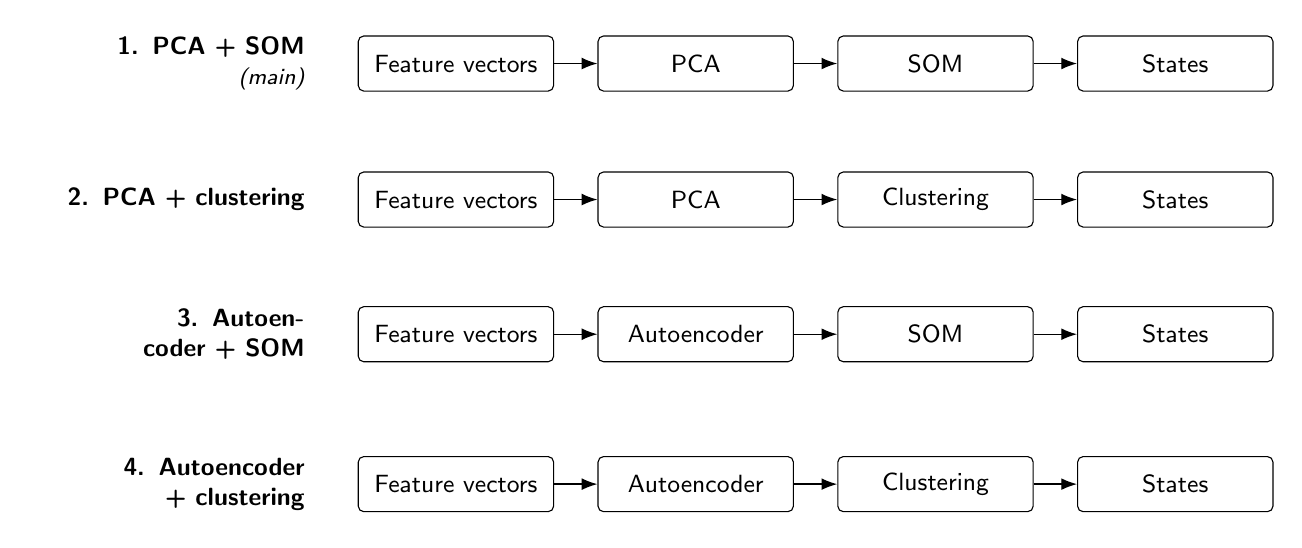
\begin{tikzpicture}[
    >={Latex[length=2mm]},
    node distance=0.45cm and 0.55cm,
    every node/.style={font=\sffamily\small},
    box/.style={
        draw, line width=0.4pt, rounded corners=2pt,
        align=center, inner sep=4pt, minimum height=0.7cm,
        text width=2.2cm
    },
    label/.style={font=\sffamily\bfseries\small, anchor=east, text width=3.4cm, align=right},
    arrow/.style={->, line width=0.5pt},
]

% --- Approach 1: PCA + SOM ---
\node[label] (l1) at (0,0) {1. PCA + SOM\\\mdseries\itshape\footnotesize (main)};
\node[box, right=of l1] (a1) {Feature vectors};
\node[box, right=of a1] (b1) {PCA};
\node[box, right=of b1] (c1) {SOM};
\node[box, right=of c1] (d1) {States};
\draw[arrow] (a1) -- (b1);
\draw[arrow] (b1) -- (c1);
\draw[arrow] (c1) -- (d1);

% --- Approach 2: PCA + clustering ---
\node[label, below=1cm of l1] (l2) {2. PCA + clustering};
\node[box, right=of l2] (a2) {Feature vectors};
\node[box, right=of a2] (b2) {PCA};
\node[box, right=of b2] (c2) {Clustering};
\node[box, right=of c2] (d2) {States};
\draw[arrow] (a2) -- (b2);
\draw[arrow] (b2) -- (c2);
\draw[arrow] (c2) -- (d2);

% --- Approach 3: Autoencoder + SOM ---
\node[label, below=1cm of l2] (l3) {3. Autoencoder + SOM};
\node[box, right=of l3] (a3) {Feature vectors};
\node[box, right=of a3] (b3) {Autoencoder};
\node[box, right=of b3] (c3) {SOM};
\node[box, right=of c3] (d3) {States};
\draw[arrow] (a3) -- (b3);
\draw[arrow] (b3) -- (c3);
\draw[arrow] (c3) -- (d3);

% --- Approach 4: Autoencoder + clustering ---
\node[label, below=1cm of l3] (l4) {4. Autoencoder + clustering};
\node[box, right=of l4] (a4) {Feature vectors};
\node[box, right=of a4] (b4) {Autoencoder};
\node[box, right=of b4] (c4) {Clustering};
\node[box, right=of c4] (d4) {States};
\draw[arrow] (a4) -- (b4);
\draw[arrow] (b4) -- (c4);
\draw[arrow] (c4) -- (d4);

\end{tikzpicture}
\caption{Pipelines for the four state-based concept drift detection approaches.
Each approach combines a dimensionality reduction step (PCA or autoencoder)
with a clustering step (SOM or k-means / similar) to produce discrete states
from per-state-type feature vectors.}
\label{fig:pipelines}
\end{figure}

% =====================================================================
\section{Implementation}
Placeholder.

% =====================================================================
\section{Evaluation}
Placeholder.

% =====================================================================
\section{Conclusion}
Placeholder.

% =====================================================================
\printbibliography

\end{document}
